
%% \documentclass{amsart}
%% \usepackage{tikz}
%% \newcommand{\scs}{\scriptsize}
%% \parindent0pt
%% \advance\textheight by1in
%% \advance\textwidth by1in
%% \advance\topmargin by-.5in
%% \advance\oddsidemargin by-.5in
%% \advance\evensidemargin by-.5in

%% \title{Small unary algebras for congruence lattices of size $\le 7$}
%% \author{Peter Jipsen}
%% \date{\today}
%% \begin{document}
%% \maketitle
Distributive lattices and lattices that are ordinal sums of smaller lattices are omitted.
The base set of each algebra is $\{0,1,\dots,n-1\}$, and each unary operation is specified by a vector of values of these elements.
Algebras of size less than $11$ are known to be minimal-size algebras that produce the corresponding congruence lattice. The algebra for
33 $(M_5)$ is also known to be minimal in size. Currently only one of the lattices (10) is not known to be the
congruence lattice of a finite algebra.

Thirteen of the 35 lattices below are subdirectly reducible (specifically: 6, 7, 12, 13, 26, 27, 28, 29, 30, 31, 32, 34, 35).
\scriptsize

\begin{tabular}{l}\begin{tikzpicture}
[scale=2, e/.style={rectangle,draw,rounded corners=3pt}]
\node(4) at (0,1)[e]{1};
\node(3) at (0.33,0.33)[e]{\begin{tikzpicture}
[scale=.3, e/.style={circle,draw,inner sep=0pt,minimum size=3pt}]
\node(a) at (0,1)[e]{};\node(b) at (1,1)[e]{};\node(c) at (0,0)[e]{};\node(d) at (1,0)[e]{};
\draw(a)--(b);\draw(c)--(d);\end{tikzpicture}};
\node(2) at (-0.5,0.0)[e]{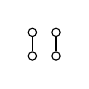
\begin{tikzpicture}
[scale=.3, e/.style={circle,draw,inner sep=0pt,minimum size=3pt}]
\node(a) at (0,1)[e]{};\node(b) at (1,1)[e]{};\node(c) at (0,0)[e]{};\node(d) at (1,0)[e]{};
\draw(a)--(c);\draw(b)--(d);\end{tikzpicture}};
\node(1) at (0.33,-0.33)[e]{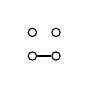
\begin{tikzpicture}
[scale=.3, e/.style={circle,draw,inner sep=0pt,minimum size=3pt}]
\node(a) at (0,1)[e]{};\node(b) at (1,1)[e]{};\node(c) at (0,0)[e]{};\node(d) at (1,0)[e]{};
\draw(c)--(d);\end{tikzpicture}};
\node(0) at (0,-1)[e]{0};
\node at (0,-1.25){\scs 1 ($N_5$)};
\node at (0,1.1)[above]{\begin{tabular}{l}
(1,0,3,2)\\
(1,0,1,0)\end{tabular}};
\node at (0,1.5){};
\draw(3)--(4);
\draw(2)--(4);
\draw(1)--(3);
\draw(0)--(1);
\draw(0)--(2);
\end{tikzpicture}\end{tabular}
\qquad\qquad
\begin{tabular}{l}\begin{tikzpicture}
[scale=2, e/.style={rectangle,draw,rounded corners=3pt}]
\node(4) at (-0.0,1.0)[e]{1};
\node(3) at (0.5,0.0)[e]{\begin{tikzpicture}
[scale=.3, e/.style={circle,draw,inner sep=0pt,minimum size=3pt}]
\node(a) at (0.5,0.87)[e]{};\node(b) at (0,0)[e]{};\node(c) at (1,0)[e]{};
\draw(a)--(b);\end{tikzpicture}};
\node(2) at (0.0,0.0)[e]{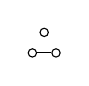
\begin{tikzpicture}
[scale=.3, e/.style={circle,draw,inner sep=0pt,minimum size=3pt}]
\node(a) at (0.5,0.87)[e]{};\node(b) at (0,0)[e]{};\node(c) at (1,0)[e]{};
\draw(b)--(c);\end{tikzpicture}};
\node(1) at (-0.5,0.0)[e]{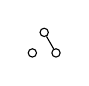
\begin{tikzpicture}
[scale=.3, e/.style={circle,draw,inner sep=0pt,minimum size=3pt}]
\node(a) at (0.5,0.87)[e]{};\node(b) at (0,0)[e]{};\node(c) at (1,0)[e]{};
\draw(a)--(c);\end{tikzpicture}};
\node(0) at (-0.0,-1.0)[e]{0};
\node at (0,-1.25){\scs 2 ($M_3$)};
\node at (0,1.1)[above]{\begin{tabular}{l}
(1,0,3,2)\\
(2,3,0,1)\end{tabular}};
\node at (0,1.5){};
\draw(3)--(4);
\draw(2)--(4);
\draw(1)--(4);
\draw(0)--(1);
\draw(0)--(2);
\draw(0)--(3);
\end{tikzpicture}\end{tabular}
\qquad\qquad
\begin{tabular}{l}\begin{tikzpicture}
[scale=2, e/.style={rectangle,draw,rounded corners=3pt}]
\node(5) at (0,1)[e]{1};
\node(4) at (0.5,0.33)[e]{\begin{tikzpicture}
[scale=.2, e/.style={circle,draw,inner sep=0pt,minimum size=2.5pt}]
\node(a) at (-1,-1)[e]{};\node(b) at (0,-1)[e]{};\node(c) at (1,-1)[e]{};\node(d) at (-1,0)[e]{};
\node(e) at (-1,1)[e]{};\node(f) at (1,0)[e]{};\node(g) at (1,1)[e]{};
\draw(d)--(a)..controls(0,-.4)..(c)--(f);\draw(e)--(g);\end{tikzpicture}};
\node(3) at (-0.5,0.0)[e]{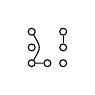
\begin{tikzpicture}
[scale=.2, e/.style={circle,draw,inner sep=0pt,minimum size=2.5pt}]
\node(a) at (-1,-1)[e]{};\node(b) at (0,-1)[e]{};\node(c) at (1,-1)[e]{};\node(d) at (-1,0)[e]{};
\node(e) at (-1,1)[e]{};\node(f) at (1,0)[e]{};\node(g) at (1,1)[e]{};
\draw(e)..controls(-.4,0)..(a)--(b);\draw(f)--(g);\end{tikzpicture}};
\node(2) at (0,0)[e]{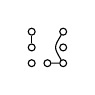
\begin{tikzpicture}
[scale=.2, e/.style={circle,draw,inner sep=0pt,minimum size=2.5pt}]
\node(a) at (-1,-1)[e]{};\node(b) at (0,-1)[e]{};\node(c) at (1,-1)[e]{};\node(d) at (-1,0)[e]{};
\node(e) at (-1,1)[e]{};\node(f) at (1,0)[e]{};\node(g) at (1,1)[e]{};
\draw(b)--(c)..controls(.4,0)..(g);\draw(d)--(e);\end{tikzpicture}};
\node(1) at (0.5,-0.33)[e]{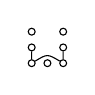
\begin{tikzpicture}
[scale=.2, e/.style={circle,draw,inner sep=0pt,minimum size=2.5pt}]
\node(a) at (-1,-1)[e]{};\node(b) at (0,-1)[e]{};\node(c) at (1,-1)[e]{};\node(d) at (-1,0)[e]{};
\node(e) at (-1,1)[e]{};\node(f) at (1,0)[e]{};\node(g) at (1,1)[e]{};
\draw(d)--(a)..controls(0,-.4)..(c)--(f);\end{tikzpicture}};
\node(0) at (0,-1)[e]{0};
\node at (0,-1.25){\scs 3 $(V_1)$};
\node at (0,1.1)[above]{\begin{tabular}{l}
$p_0=$ (0,1,2,1,2,1,0)\\
$p_1=$ (0,3,4,3,4,3,0)\\
$p_2=$ (6,5,2,5,2,5,6)\\
$p_3=$ (0,1,2,0,0,2,2)\end{tabular}};
\node at (0,1.5){};
\draw(4)--(5);
\draw(3)--(5);
\draw(2)--(5);
\draw(1)--(4);
\draw(0)--(1);
\draw(0)--(2);
\draw(0)--(3);
\end{tikzpicture}\end{tabular}
%\end{document}
%#4 [[1,2,3,4,5,0,7,8,9,10,11,6], #D12 + 2-elt range
%[6,11,10,9,8,7,0,5,4,3,2,1],
%[0,0,0,6,0,0,0,0,6,0,0,0]])
%#5 [[1,0,3,2],[0,0,2,2]])
%#6 [[2,2,1,5,5,4],[3,4,4,0,1,1],[4,5,3,4,5,3]])
%#7 [[1,0,0,4,3,3],[4,5,5,1,2,2],[3,3,4,3,3,4]])
%#8 [[1,2,0,4,5,3],[3,5,4,0,2,1]])
%#9 [[0,0,0,0,0,0,2,1,2,1,3,4,5,3,4,5], 
%[0,0,0,0,0,0,6,7,6,7,10,11,12,10,11,12], 
%[13,14,15,1,9,8,15,14,13,15,1,9,8,8,1,9]]
%#10 No finite algebra known with this congruence lattice
%#11 #algebra from filter-ideal in upper interval of SmallGroup(216,153) found by William Demeo using GAP
%#108 elements (not known to be the smallest)
%#12 [[0,0,3,3,3,6,6,6,0],[0,0,8,8,8,1,1,1,0],[0,5,5,4,0,0,5,4,4],[4,2,2,3,4,4,2,3,3],[5,5,7,7,7,6,6,6,5]])
%#13 [
%( 0, 1, 2, 0, 0, 2, 2, 0, 3, 4, 0, 4, 4, 6, 5, 2, 6, 6, 2), 
%( 0, 1, 2, 3, 4, 5, 6, 0, 1, 2, 4, 5, 6, 0, 1, 2, 3, 4, 6), 
%( 7, 8, 9, 3,10,11,12, 3, 3, 3, 3, 3, 3,11,11,11,11,11,11), 
%(13,14,15,16,17, 5,18,13,16,17,17,16,13, 5, 5, 5, 5, 5, 5),
%( 0, 1, 2, 1, 2, 1, 0, 0, 1, 2, 2, 1, 0, 0, 1, 2, 1, 2, 0)])
%#14 (dual of #15)
%#no explicit small representation known?
%#15 [[1,0,3,2]]
%#16 (dual of #17)
%#no explicit small representation known?
%#17 ((M_3+1)||1)
%#representation from filter-ideal of Sub(A_4)
%[(1,0,3,2,5,4,7,6,9,8,11,10),
%(4,7,5,6,8,11,9,10,0,3,1,2),
%(0,0,0,0,5,5,5,5,10,10,10,10)]
%#18 (dual of #19)
%#no explicit small representation known?
%#19
%#representation found by search in Equ(8) by Peter (smallest)
%[(0,1,1,0,4,5,5,4),
%(0,2,3,1,0,2,3,1),
%(7,6,6,7,3,2,2,3)])
%#20
%#representation found by William Demeo in SmallGroup(216,153)
%#21
%#representation found by Ralph Freese searching through Equ(10)
%#22 (dual of #23)
%#no explicit small representation known?
%#23
%#representation found by searching through Equ(6)
%[(0,1,0,1,4,4), (1,1,3,3,4,5), (3,2,3,2,5,5), (4,1,5,3,4,5)]
%#24 (L_2 in Jonsson-Rival 1979)
%#representation found by searching through Equ(6)
%[(1,1,2,2), (2,3,3,2)]
%#25 (L_1 in Jonsson-Rival 1979)
%[(0, 0, 2, 2, 2), (0, 1, 0, 1, 1), (1, 1, 4, 4, 4), (2, 3, 2, 3, 3)]
%#26 [(1, 0, 3, 2, 0, 2), (4, 4, 5, 5, 1, 3),(0, 0, 0, 0, 1, 1), (3, 5, 3, 5, 3, 3)]
%#27 (4||5)
%#representation from rabbit ears construction applied to #6. |A|=16 (not known to be smallest)
%[
%[ 0, 6, 7, 8, 9,10, 6, 7, 8, 9,10, 0, 6, 8, 9,10], 
%[11,12, 2,13,14,15,12, 2,13,14,15,11,12,13,14,15], 
%[ 0, 1, 2, 3, 4, 5, 0, 0, 0, 0, 0, 2, 2, 2, 2, 2], 
%[ 4, 5, 3, 4, 5, 3, 5, 3, 4, 5, 3, 4, 5, 4, 5, 3], 
%[ 2, 2, 1, 5, 5, 4, 2, 1, 5, 5, 4, 2, 2, 5, 5, 4], 
%[ 3, 4, 4, 0, 1, 1, 4, 4, 0, 1, 1, 3, 4, 0, 1, 1]]
%
%
\qquad\qquad
\begin{tabular}{l}\begin{tikzpicture}
[scale=2, e/.style={rectangle,draw,rounded corners=3pt}]
\node(5) at (0,1)[e]{1};
\node(4) at (0,0.33)[e]{\begin{tikzpicture}
[scale=.2, e/.style={circle,draw,inner sep=0pt,minimum size=3pt}]
\node(a) at (0,1.2)[e]{};\node(b) at (1,1.2)[e]{};\node(c) at (2,1.2)[e]{};\node(d) at (3,1.2)[e]{};
\node(e) at (4,1.2)[e]{};\node(f) at (5,1.2)[e]{};\node(g) at (0,0)[e]{};\node(h) at (1,0)[e]{};
\node(i) at (2,0)[e]{};\node(j) at (3,0)[e]{};\node(k) at (4,0)[e]{};\node(l) at (5,0)[e]{};
\draw(a)--(b)--(c)--(d)--(e)--(f);\draw(g)--(h)--(i)--(j)--(k)--(l);\end{tikzpicture}};
\node(3) at (1,0.33)[e]{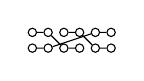
\begin{tikzpicture}
[scale=.2, e/.style={circle,draw,inner sep=0pt,minimum size=3pt}]
\node(a) at (0,1)[e]{};\node(b) at (1,1)[e]{};\node(c) at (2,1)[e]{};\node(d) at (3,1)[e]{};
\node(e) at (4,1)[e]{};\node(f) at (5,1)[e]{};\node(g) at (0,0)[e]{};\node(h) at (1,0)[e]{};
\node(i) at (2,0)[e]{};\node(j) at (3,0)[e]{};\node(k) at (4,0)[e]{};\node(l) at (5,0)[e]{};
\draw(a)--(b)--(i)--(j);\draw(c)--(d)--(k)--(l);\draw(g)--(h)--(e)--(f);\end{tikzpicture}};
\node(2) at (-0.75,0)[e]{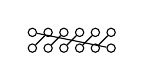
\begin{tikzpicture}
[scale=.2, e/.style={circle,draw,inner sep=0pt,minimum size=3pt}]
\node(a) at (0,1)[e]{};\node(b) at (1,1)[e]{};\node(c) at (2,1)[e]{};\node(d) at (3,1)[e]{};
\node(e) at (4,1)[e]{};\node(f) at (5,1)[e]{};\node(g) at (0,0)[e]{};\node(h) at (1,0)[e]{};
\node(i) at (2,0)[e]{};\node(j) at (3,0)[e]{};\node(k) at (4,0)[e]{};\node(l) at (5,0)[e]{};
\draw(a)--(l);\draw(b)--(g);\draw(c)--(h);\draw(d)--(i);\draw(e)--(j);\draw(f)--(k);\end{tikzpicture}};
\node(1) at (0.5,-0.33)[e]{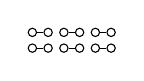
\begin{tikzpicture}
[scale=.2, e/.style={circle,draw,inner sep=0pt,minimum size=3pt}]
\node(a) at (0,1)[e]{};\node(b) at (1,1)[e]{};\node(c) at (2,1)[e]{};\node(d) at (3,1)[e]{};
\node(e) at (4,1)[e]{};\node(f) at (5,1)[e]{};\node(g) at (0,0)[e]{};\node(h) at (1,0)[e]{};
\node(i) at (2,0)[e]{};\node(j) at (3,0)[e]{};\node(k) at (4,0)[e]{};\node(l) at (5,0)[e]{};
\draw(a)--(b);\draw(c)--(d);\draw(e)--(f);\draw(g)--(h);\draw(i)--(j);\draw(k)--(l);\end{tikzpicture}};
\node(0) at (0,-1)[e]{0};
\node at (0,-1.25){\scs 4 $(L_5)$};
\node at (0,1.1)[above]{\begin{tabular}{l}
(1,2,3,4,5,0,7,8,9,10,11,6)\\
(6,11,10,9,8,7,0,5,4,3,2,1)\\
(0,\phantom{1}0,\phantom{1}0,6,0,0,0,0,6,0,0,0)\end{tabular}};
\node at (0,1.5){};
\draw(4)--(5);
\draw(3)--(5);
\draw(2)--(5);
\draw(1)--(3);
\draw(1)--(4);
\draw(0)--(1);
\draw(0)--(2);
\end{tikzpicture}\end{tabular}
\qquad\qquad
\begin{tabular}{l}\begin{tikzpicture}
[scale=2, e/.style={rectangle,draw,rounded corners=3pt}]
\node(5) at (0,1)[e]{1};
\node(4) at (0.2,0.33)[e]{\begin{tikzpicture}
[scale=.3, e/.style={circle,draw,inner sep=0pt,minimum size=3pt}]
\node(a) at (0,1)[e]{};\node(b) at (1,1)[e]{};\node(c) at (0,0)[e]{};\node(d) at (1,0)[e]{};
\draw(a)--(b);\draw(c)--(d);\end{tikzpicture}};
\node(3) at (-0.5,0)[e]{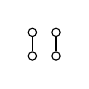
\begin{tikzpicture}
[scale=.3, e/.style={circle,draw,inner sep=0pt,minimum size=3pt}]
\node(a) at (0,1)[e]{};\node(b) at (1,1)[e]{};\node(c) at (0,0)[e]{};\node(d) at (1,0)[e]{};
\draw(a)--(c);\draw(b)--(d);\end{tikzpicture}};
\node(2) at (0.34,-0.33)[e]{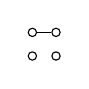
\begin{tikzpicture}
[scale=.3, e/.style={circle,draw,inner sep=0pt,minimum size=3pt}]
\node(a) at (0,1)[e]{};\node(b) at (1,1)[e]{};\node(c) at (0,0)[e]{};\node(d) at (1,0)[e]{};
\draw(a)--(b);\end{tikzpicture}};
\node(1) at (0,-0.33)[e]{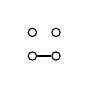
\begin{tikzpicture}
[scale=.3, e/.style={circle,draw,inner sep=0pt,minimum size=3pt}]
\node(a) at (0,1)[e]{};\node(b) at (1,1)[e]{};\node(c) at (0,0)[e]{};\node(d) at (1,0)[e]{};
\draw(c)--(d);\end{tikzpicture}};
\node(0) at (0,-1)[e]{0};
\node at (0,-1.25){\scs 5 $(L_4)$};
\node at (0,1.1)[above]{\begin{tabular}{l}
(1,0,3,2)\\ 
(0,0,2,2)\end{tabular}};
\node at (0,1.5){};
\draw(4)--(5);
\draw(3)--(5);
\draw(2)--(4);
\draw(1)--(4);
\draw(0)--(3);
\draw(0)--(2);
\draw(0)--(1);
\end{tikzpicture}\end{tabular}
\qquad\qquad
\begin{tabular}{l}\begin{tikzpicture}
[scale=2, e/.style={rectangle,draw,rounded corners=3pt}]
\node(5) at (0,1)[e]{1};
\node(4) at (-0.5,0.33)[e]{\begin{tikzpicture}
[scale=.3, e/.style={circle,draw,inner sep=0pt,minimum size=3pt}]
\node(a) at (0,1)[e]{};\node(b) at (1,1)[e]{};\node(c) at (2,1)[e]{};\node(d) at (0,0)[e]{};\node(e) at (1,0)[e]{};\node(f) at (2,0)[e]{};
\draw(a)--(d);\draw(b)--(e);\draw(c)--(f);\end{tikzpicture}};
\node(3) at (0.5,0.33)[e]{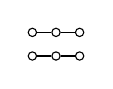
\begin{tikzpicture}
[scale=.3, e/.style={circle,draw,inner sep=0pt,minimum size=3pt}]
\node(a) at (0,1)[e]{};\node(b) at (1,1)[e]{};\node(c) at (2,1)[e]{};\node(d) at (0,0)[e]{};\node(e) at (1,0)[e]{};\node(f) at (2,0)[e]{};
\draw(a)--(b)--(c);\draw(d)--(e)--(f);\end{tikzpicture}};
\node(2) at (-0.5,-0.33)[e]{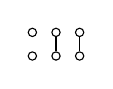
\begin{tikzpicture}
[scale=.3, e/.style={circle,draw,inner sep=0pt,minimum size=3pt}]
\node(a) at (0,1)[e]{};\node(b) at (1,1)[e]{};\node(c) at (2,1)[e]{};\node(d) at (0,0)[e]{};\node(e) at (1,0)[e]{};\node(f) at (2,0)[e]{};
\draw(b)--(e);\draw(c)--(f);\end{tikzpicture}};
\node(1) at (0.5,-0.33)[e]{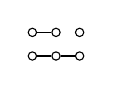
\begin{tikzpicture}
[scale=.3, e/.style={circle,draw,inner sep=0pt,minimum size=3pt}]
\node(a) at (0,1)[e]{};\node(b) at (1,1)[e]{};\node(c) at (2,1)[e]{};\node(d) at (0,0)[e]{};\node(e) at (1,0)[e]{};\node(f) at (2,0)[e]{};
\draw(a)--(b);\draw(d)--(e)--(f);\end{tikzpicture}};
\node(0) at (0,-1)[e]{0};
\node at (0,-1.25){\scs 6};
\node at (0,1.1)[above]{\begin{tabular}{l}
(2,2,1,5,5,4)\\
(3,4,4,0,1,1)\\
(4,5,3,4,5,3)\end{tabular}};
\node at (0,1.5){};
\draw(4)--(5);
\draw(3)--(5);
\draw(2)--(4);
\draw(1)--(3);
\draw(0)--(1);
\draw(0)--(2);
\end{tikzpicture}\end{tabular}
\qquad\qquad
\begin{tabular}{l}\begin{tikzpicture}
[scale=2, e/.style={rectangle,draw,rounded corners=3pt}]
\node(5) at (0,1)[e]{1};
\node(4) at (0.5,0.5)[e]{\begin{tikzpicture}
[scale=.3, e/.style={circle,draw,inner sep=0pt,minimum size=3pt}]
\node(a) at (0,1)[e]{};\node(b) at (1,1)[e]{};\node(c) at (2,1)[e]{};\node(d) at (0,0)[e]{};\node(e) at (1,0)[e]{};\node(f) at (2,0)[e]{};
\draw(a)--(b)--(c);\draw(d)--(e)--(f);\end{tikzpicture}};
\node(3) at (-0.5,0)[e]{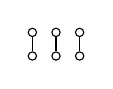
\begin{tikzpicture}
[scale=.3, e/.style={circle,draw,inner sep=0pt,minimum size=3pt}]
\node(a) at (0,1)[e]{};\node(b) at (1,1)[e]{};\node(c) at (2,1)[e]{};\node(d) at (0,0)[e]{};\node(e) at (1,0)[e]{};\node(f) at (2,0)[e]{};
\draw(a)--(d);\draw(b)--(e);\draw(c)--(f);\end{tikzpicture}};
\node(2) at (0.5,0)[e]{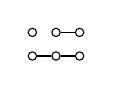
\begin{tikzpicture}
[scale=.3, e/.style={circle,draw,inner sep=0pt,minimum size=3pt}]
\node(a) at (0,1)[e]{};\node(b) at (1,1)[e]{};\node(c) at (2,1)[e]{};\node(d) at (0,0)[e]{};\node(e) at (1,0)[e]{};\node(f) at (2,0)[e]{};
\draw(b)--(c);\draw(d)--(e)--(f);\end{tikzpicture}};
\node(1) at (0.5,-0.5)[e]{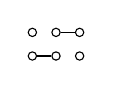
\begin{tikzpicture}
[scale=.3, e/.style={circle,draw,inner sep=0pt,minimum size=3pt}]
\node(a) at (0,1)[e]{};\node(b) at (1,1)[e]{};\node(c) at (2,1)[e]{};\node(d) at (0,0)[e]{};\node(e) at (1,0)[e]{};\node(f) at (2,0)[e]{};
\draw(b)--(c);\draw(d)--(e);\end{tikzpicture}};
\node(0) at (0,-1)[e]{0};
\node at (0,-1.25){\scs 7};
\node at (0,1.1)[above]{\begin{tabular}{l}
(1,0,0,4,3,3)\\
(4,5,5,1,2,2)\\
(3,3,4,3,3,4)\end{tabular}};
\node at (0,1.5){};
\draw(4)--(5);
\draw(3)--(5);
\draw(2)--(4);
\draw(1)--(2);
\draw(0)--(1);
\draw(0)--(3);
\end{tikzpicture}\end{tabular}
\qquad\qquad
\begin{tabular}{l}\begin{tikzpicture}
[scale=2, e/.style={rectangle,draw,rounded corners=3pt}]
\node(5) at (0,1)[e]{1};
\node(4) at (-1,0.0)[e]{\begin{tikzpicture}
[scale=.3, e/.style={circle,draw,inner sep=0pt,minimum size=3pt}]
\node(a) at (0,1)[e]{};\node(b) at (1,1)[e]{};\node(c) at (2,1)[e]{};\node(d) at (0,0)[e]{};\node(e) at (1,0)[e]{};\node(f) at (2,0)[e]{};
\draw(a)--(b)--(c);\draw(d)--(e)--(f);\end{tikzpicture}};
\node(3) at (-.33,0)[e]{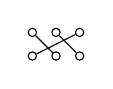
\begin{tikzpicture}
[scale=.3, e/.style={circle,draw,inner sep=0pt,minimum size=3pt}]
\node(a) at (0,1)[e]{};\node(b) at (1,1)[e]{};\node(c) at (2,1)[e]{};\node(d) at (0,0)[e]{};\node(e) at (1,0)[e]{};\node(f) at (2,0)[e]{};
\draw(a)--(e);\draw(b)--(f);\draw(c)--(d);\end{tikzpicture}};
\node(2) at (0.33,0)[e]{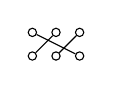
\begin{tikzpicture}
[scale=.3, e/.style={circle,draw,inner sep=0pt,minimum size=3pt}]
\node(a) at (0,1)[e]{};\node(b) at (1,1)[e]{};\node(c) at (2,1)[e]{};\node(d) at (0,0)[e]{};\node(e) at (1,0)[e]{};\node(f) at (2,0)[e]{};
\draw(a)--(f);\draw(b)--(d);\draw(c)--(e);\end{tikzpicture}};
\node(1) at (1,0)[e]{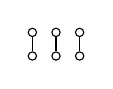
\begin{tikzpicture}
[scale=.3, e/.style={circle,draw,inner sep=0pt,minimum size=3pt}]
\node(a) at (0,1)[e]{};\node(b) at (1,1)[e]{};\node(c) at (2,1)[e]{};\node(d) at (0,0)[e]{};\node(e) at (1,0)[e]{};\node(f) at (2,0)[e]{};
\draw(a)--(d);\draw(b)--(e);\draw(c)--(f);\end{tikzpicture}};
\node(0) at (0,-1)[e]{0};
\node at (0,-1.25){\scs 8 $(M_4)$};
\node at (0,1.1)[above]{\begin{tabular}{l}
(1,2,0,4,5,3)\\
(3,5,4,0,2,1)\end{tabular}};
\node at (0,1.5){};
\draw(4)--(5);
\draw(3)--(5);
\draw(2)--(5);
\draw(1)--(5);
\draw(0)--(1);
\draw(0)--(2);
\draw(0)--(3);
\draw(0)--(4);
\end{tikzpicture}\end{tabular}
\begin{tabular}{l}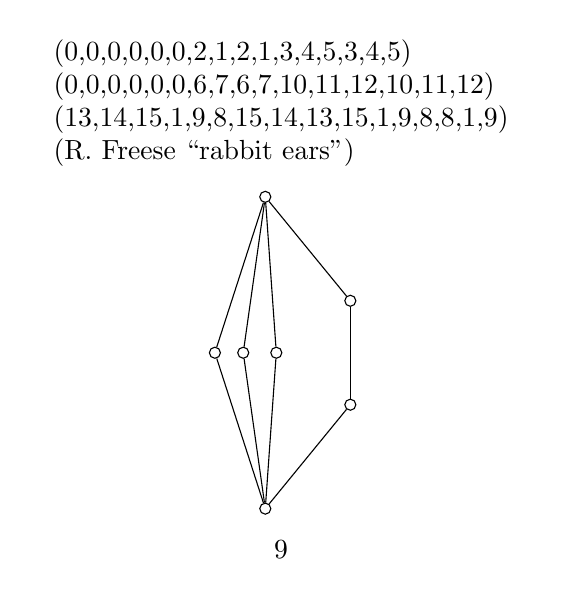
\begin{tikzpicture}
[scale=2, e/.style={circle,draw,inner sep=0pt,minimum size=4pt}]
\node(6) at (-0.1,0.99)[e]{};
\node(5) at (0.44,0.33)[e]{};
\node(4) at (-0.24,0.0)[e]{};
\node(3) at (-0.42,0.0)[e]{};
\node(2) at (-0.03,0.0)[e]{};
\node(1) at (0.44,-0.33)[e]{};
\node(0) at (-0.1,-0.99)[e]{};
\node at (0,-1.25){\scs 9};
\node at (0,1.1)[above]{\begin{tabular}{l}
(0,0,0,0,0,0,2,1,2,1,3,4,5,3,4,5)\\
(0,0,0,0,0,0,6,7,6,7,10,11,12,10,11,12)\\ 
(13,14,15,1,9,8,15,14,13,15,1,9,8,8,1,9)\\
(R. Freese ``rabbit ears'')
\end{tabular}};
\node at (0,1.5){};
\draw(5)--(6);
\draw(4)--(6);
\draw(3)--(6);
\draw(2)--(6);
\draw(1)--(5);
\draw(0)--(1);
\draw(0)--(2);
\draw(0)--(3);
\draw(0)--(4);
\end{tikzpicture}\end{tabular}
\begin{tabular}{l}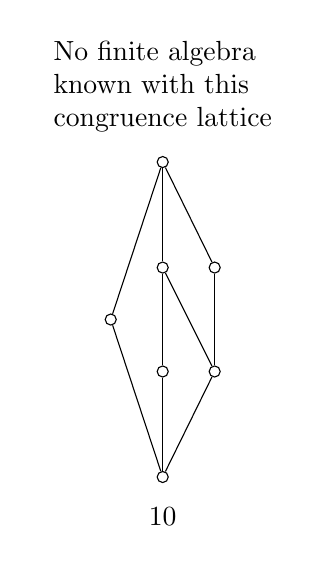
\begin{tikzpicture}
[scale=2, e/.style={circle,draw,inner sep=0pt,minimum size=4pt}]
\node(6) at (0,1)[e]{};
\node(5) at (0,0.33)[e]{};
\node(4) at (0.33,0.33)[e]{};
\node(3) at (-0.33,0.0)[e]{};
\node(2) at (0,-0.33)[e]{};
\node(1) at (0.33,-0.33)[e]{};
\node(0) at (0,-1)[e]{};
\node at (0,-1.25){\scs 10};
\node at (0,1.1)[above]{\begin{tabular}{l}
No finite algebra\\
known with this\\
congruence lattice\end{tabular}};
\node at (0,1.5){};
\draw(5)--(6);
\draw(4)--(6);
\draw(3)--(6);
\draw(2)--(5);
\draw(1)--(4);
\draw(1)--(5);
\draw(0)--(1);
\draw(0)--(2);
\draw(0)--(3);
\end{tikzpicture}\end{tabular}
\begin{tabular}{l}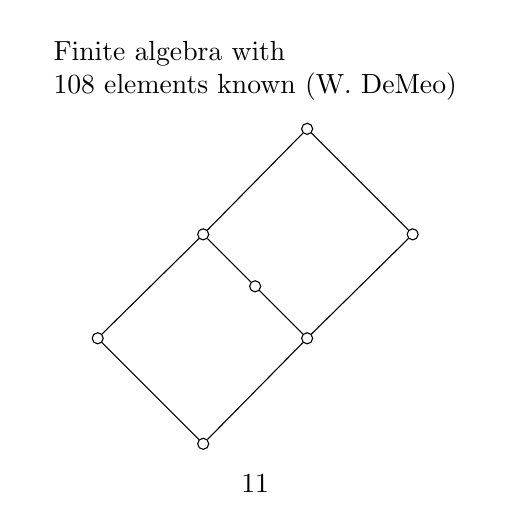
\begin{tikzpicture}
[scale=2, e/.style={circle,draw,inner sep=0pt,minimum size=4pt}]
\node(6) at (0.33,1)[e]{};
\node(5) at (-0.33,0.33)[e]{};
\node(4) at (1,0.33)[e]{};
\node(3) at (0,0)[e]{};
\node(2) at (-1,-0.33)[e]{};
\node(1) at (0.33,-0.33)[e]{};
\node(0) at (-0.33,-1)[e]{};
\node at (0,-1.25){\scs 11};
\node at (0,1.1)[above]{\begin{tabular}{l}
Finite algebra with\\
108 elements known (W. DeMeo)\end{tabular}};
\node at (0,1.5){};
\draw(5)--(6);
\draw(4)--(6);
\draw(3)--(5);
\draw(2)--(5);
\draw(1)--(3);
\draw(1)--(4);
\draw(0)--(1);
\draw(0)--(2);
\end{tikzpicture}\end{tabular}
\begin{tabular}{l}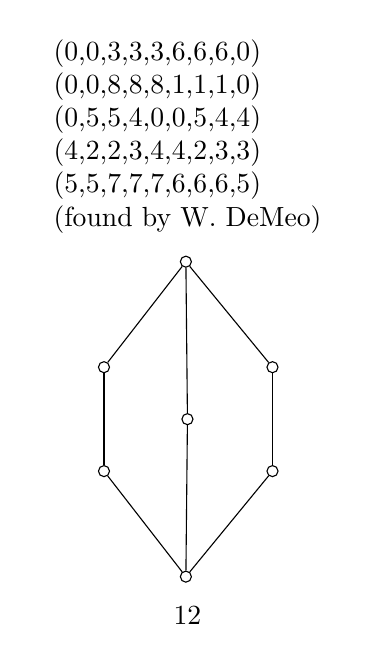
\begin{tikzpicture}
[scale=2, e/.style={circle,draw,inner sep=0pt,minimum size=4pt}]
\node(6) at (-0.01,1.0)[e]{};
\node(5) at (0.54,0.33)[e]{};
\node(4) at (-0.53,0.33)[e]{};
\node(3) at (0.0,0.0)[e]{};
\node(2) at (0.54,-0.33)[e]{};
\node(1) at (-0.53,-0.33)[e]{};
\node(0) at (-0.01,-1.0)[e]{};
\node at (0,-1.25){\scs 12 };
\node at (0,1.1)[above]{\begin{tabular}{l}
(0,0,3,3,3,6,6,6,0)\\
(0,0,8,8,8,1,1,1,0)\\
(0,5,5,4,0,0,5,4,4)\\
(4,2,2,3,4,4,2,3,3)\\
(5,5,7,7,7,6,6,6,5)\\
(found by W. DeMeo)\end{tabular}};
\node at (0,1.5){};
\draw(5)--(6);
\draw(4)--(6);
\draw(3)--(6);
\draw(2)--(5);
\draw(1)--(4);
\draw(0)--(1);
\draw(0)--(2);
\draw(0)--(3);
\end{tikzpicture}\end{tabular}
\begin{tabular}{l}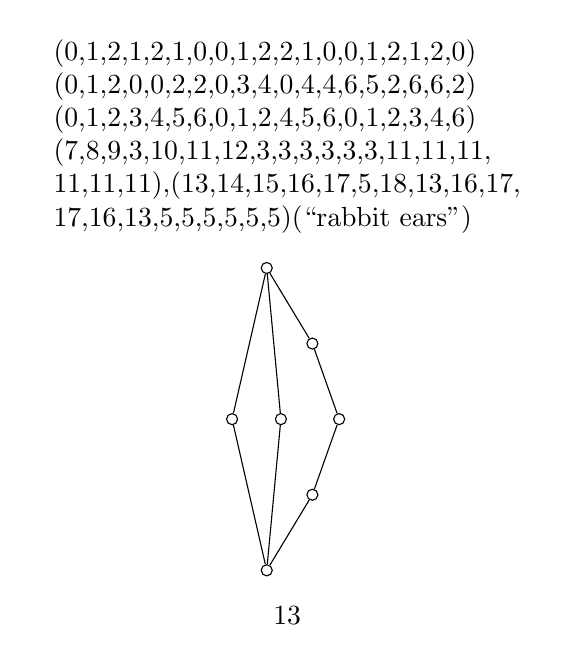
\begin{tikzpicture}
[scale=2, e/.style={circle,draw,inner sep=0pt,minimum size=4pt}]
\node(6) at (-0.13,0.96)[e]{};
\node(5) at (0.16,0.48)[e]{};
\node(4) at (-0.04,0.0)[e]{};
\node(3) at (-0.35,0.0)[e]{};
\node(2) at (0.33,0.0)[e]{};
\node(1) at (0.16,-0.48)[e]{};
\node(0) at (-0.13,-0.96)[e]{};
\node at (0,-1.25){\scs 13 };
\node at (0,1.1)[above]{\begin{tabular}{l}
(0,1,2,1,2,1,0,0,1,2,2,1,0,0,1,2,1,2,0)\\
(0,1,2,0,0,2,2,0,3,4,0,4,4,6,5,2,6,6,2)\\
(0,1,2,3,4,5,6,0,1,2,4,5,6,0,1,2,3,4,6)\\
(7,8,9,3,10,11,12,3,3,3,3,3,3,11,11,11,\\
11,11,11),(13,14,15,16,17,5,18,13,16,17,\\
17,16,13,5,5,5,5,5,5)(``rabbit ears'')\end{tabular}};
\node at (0,1.5){};
\draw(5)--(6);
\draw(4)--(6);
\draw(3)--(6);
\draw(2)--(5);
\draw(1)--(2);
\draw(0)--(1);
\draw(0)--(3);
\draw(0)--(4);
\end{tikzpicture}\end{tabular}
\begin{tabular}{l}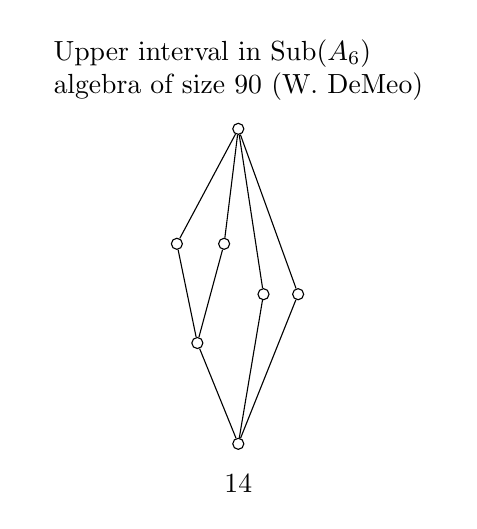
\begin{tikzpicture}
[scale=2, e/.style={circle,draw,inner sep=0pt,minimum size=4pt}]
\node(6) at (0,1)[e]{};
\node(5) at (-0.39,0.27)[e]{};
\node(4) at (-0.09,0.27)[e]{};
\node(3) at (0.38,-0.05)[e]{};
\node(2) at (0.16,-0.05)[e]{};
\node(1) at (-0.26,-0.36)[e]{};
\node(0) at (0,-1)[e]{};
\node at (0,-1.25){\scs 14};
\node at (0,1.1)[above]{\begin{tabular}{l}
Upper interval in Sub$(A_6)$\\
algebra of size 90 (W. DeMeo)\end{tabular}};
\node at (0,1.5){};
\draw(5)--(6);
\draw(4)--(6);
\draw(3)--(6);
\draw(2)--(6);
\draw(1)--(4);
\draw(1)--(5);
\draw(0)--(1);
\draw(0)--(2);
\draw(0)--(3);
\end{tikzpicture}\end{tabular}
\begin{tabular}{l}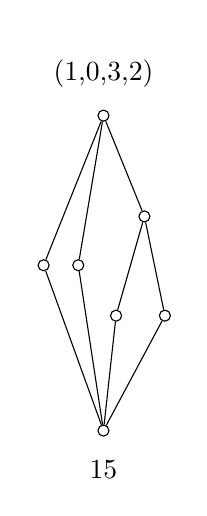
\begin{tikzpicture}
[scale=2, e/.style={circle,draw,inner sep=0pt,minimum size=4pt}]
\node(6) at (0,1)[e]{};
\node(5) at (0.26,0.36)[e]{};
\node(4) at (-0.16,0.05)[e]{};
\node(3) at (-0.38,0.05)[e]{};
\node(2) at (0.08,-0.27)[e]{};
\node(1) at (0.39,-0.27)[e]{};
\node(0) at (0,-1)[e]{};
\node at (0,-1.25){\scs 15};
\node at (0,1.1)[above]{\begin{tabular}{l}
(1,0,3,2)\end{tabular}};
\node at (0,1.5){};
\draw(5)--(6);
\draw(4)--(6);
\draw(3)--(6);
\draw(2)--(5);
\draw(1)--(5);
\draw(0)--(4);
\draw(0)--(3);
\draw(0)--(2);
\draw(0)--(1);
\end{tikzpicture}\end{tabular}
\begin{tabular}{l}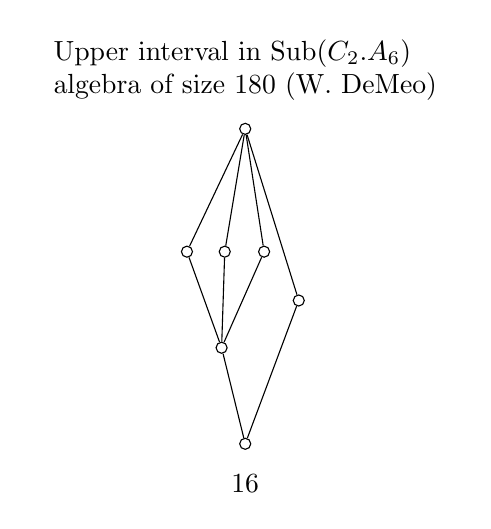
\begin{tikzpicture}
[scale=2, e/.style={circle,draw,inner sep=0pt,minimum size=4pt}]
\node(6) at (0,1)[e]{};
\node(5) at (0.12,0.22)[e]{};
\node(4) at (-0.37,0.22)[e]{};
\node(3) at (-0.13,0.22)[e]{};
\node(2) at (0.34,-0.09)[e]{};
\node(1) at (-0.15,-0.39)[e]{};
\node(0) at (0,-1)[e]{};
\node at (0,-1.25){\scs 16};
\node at (0,1.1)[above]{\begin{tabular}{l}
Upper interval in Sub$(C_2.A_6)$\\
algebra of size 180 (W. DeMeo)\end{tabular}};
\node at (0,1.5){};
\draw(5)--(6);
\draw(4)--(6);
\draw(3)--(6);
\draw(2)--(6);
\draw(1)--(3);
\draw(1)--(4);
\draw(1)--(5);
\draw(0)--(1);
\draw(0)--(2);
\end{tikzpicture}\end{tabular}
\begin{tabular}{l}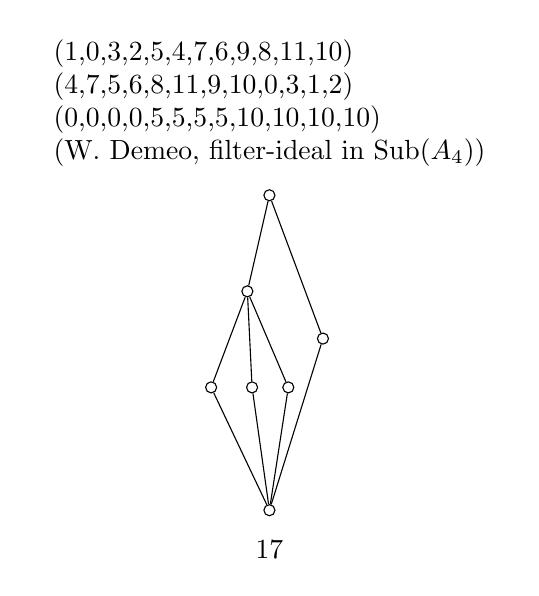
\begin{tikzpicture}
[scale=2, e/.style={circle,draw,inner sep=0pt,minimum size=4pt}]
\node(6) at (0,1.0)[e]{};
\node(5) at (-0.14,0.39)[e]{};
\node(4) at (0.34,0.09)[e]{};
\node(3) at (0.12,-0.22)[e]{};
\node(2) at (-0.11,-0.22)[e]{};
\node(1) at (-0.37,-0.22)[e]{};
\node(0) at (0,-1)[e]{};
\node at (0,-1.25){\scs 17};
\node at (0,1.1)[above]{\begin{tabular}{l}
(1,0,3,2,5,4,7,6,9,8,11,10)\\
(4,7,5,6,8,11,9,10,0,3,1,2)\\
(0,0,0,0,5,5,5,5,10,10,10,10)\\
(W. Demeo, filter-ideal in Sub$(A_4)$)\end{tabular}};
\node at (0,1.5){};
\draw(5)--(6);
\draw(4)--(6);
\draw(3)--(5);
\draw(2)--(5);
\draw(1)--(5);
\draw(0)--(4);
\draw(0)--(3);
\draw(0)--(2);
\draw(0)--(1);
\end{tikzpicture}\end{tabular}
\begin{tabular}{l}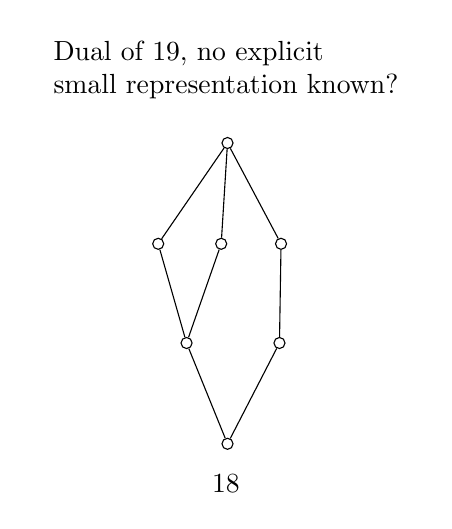
\begin{tikzpicture}
[scale=2, e/.style={circle,draw,inner sep=0pt,minimum size=4pt}]
\node(6) at (0.01,0.91)[e]{};
\node(5) at (0.35,0.27)[e]{};
\node(4) at (-0.43,0.27)[e]{};
\node(3) at (-0.03,0.27)[e]{};
\node(2) at (0.34,-0.36)[e]{};
\node(1) at (-0.25,-0.36)[e]{};
\node(0) at (0.01,-1.0)[e]{};
\node at (0,-1.25){\scs 18};
\node at (0,1.1)[above]{\begin{tabular}{l}
Dual of 19, no explicit\\
small representation known?\end{tabular}};
\node at (0,1.5){};
\draw(5)--(6);
\draw(4)--(6);
\draw(3)--(6);
\draw(2)--(5);
\draw(1)--(3);
\draw(1)--(4);
\draw(0)--(1);
\draw(0)--(2);
\end{tikzpicture}\end{tabular}
\begin{tabular}{l}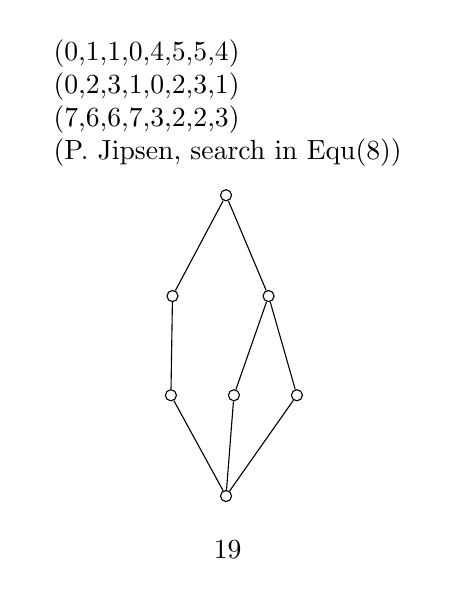
\begin{tikzpicture}
[scale=2, e/.style={circle,draw,inner sep=0pt,minimum size=4pt}]
\node(6) at (-0.01,1.0)[e]{};
\node(5) at (0.26,0.36)[e]{};
\node(4) at (-0.35,0.36)[e]{};
\node(3) at (0.44,-0.27)[e]{};
\node(2) at (0.04,-0.27)[e]{};
\node(1) at (-0.36,-0.27)[e]{};
\node(0) at (-0.01,-0.91)[e]{};
\node at (0,-1.25){\scs 19};
\node at (0,1.1)[above]{\begin{tabular}{l}
(0,1,1,0,4,5,5,4)\\
(0,2,3,1,0,2,3,1)\\
(7,6,6,7,3,2,2,3)\\
(P. Jipsen, search in Equ(8))
\end{tabular}};
\node at (0,1.5){};
\draw(5)--(6);
\draw(4)--(6);
\draw(3)--(5);
\draw(2)--(5);
\draw(1)--(4);
\draw(0)--(3);
\draw(0)--(2);
\draw(0)--(1);
\end{tikzpicture}\end{tabular}
\begin{tabular}{l}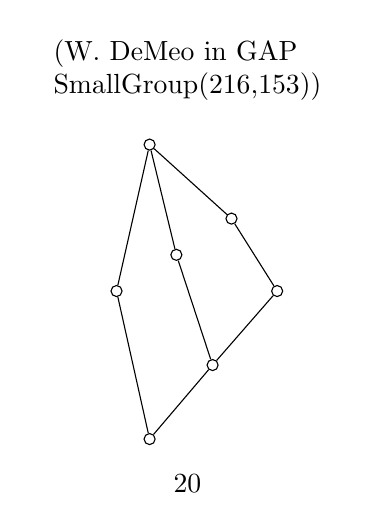
\begin{tikzpicture}
[scale=2, e/.style={circle,draw,inner sep=0pt,minimum size=4pt}]
\node(6) at (-0.24,0.9)[e]{};
\node(5) at (0.28,0.43)[e]{};
\node(4) at (-0.07,0.2)[e]{};
\node(3) at (-0.45,-0.03)[e]{};
\node(2) at (0.57,-0.03)[e]{};
\node(1) at (0.16,-0.5)[e]{};
\node(0) at (-0.24,-0.97)[e]{};
\node at (0,-1.25){\scs 20};
\node at (0,1.1)[above]{\begin{tabular}{l}
(W. DeMeo in GAP \\
SmallGroup(216,153))\end{tabular}};
\node at (0,1.5){};
\draw(5)--(6);
\draw(4)--(6);
\draw(3)--(6);
\draw(2)--(5);
\draw(1)--(2);
\draw(1)--(4);
\draw(0)--(1);
\draw(0)--(3);
\end{tikzpicture}\end{tabular}
\begin{tabular}{l}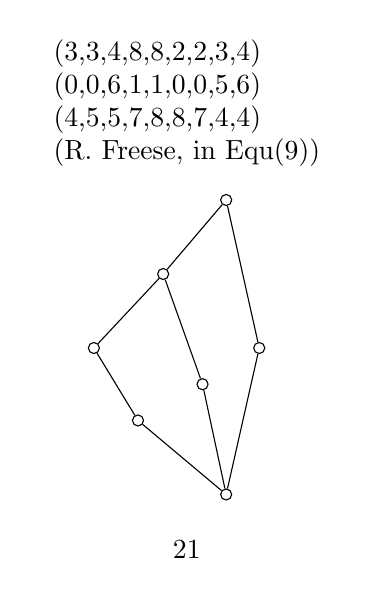
\begin{tikzpicture}
[scale=2, e/.style={circle,draw,inner sep=0pt,minimum size=4pt}]
\node(6) at (0.25,0.97)[e]{};
\node(5) at (-0.15,0.5)[e]{};
\node(4) at (-0.59,0.03)[e]{};
\node(3) at (0.46,0.03)[e]{};
\node(2) at (0.1,-0.2)[e]{};
\node(1) at (-0.31,-0.43)[e]{};
\node(0) at (0.25,-0.9)[e]{};
\node at (0,-1.25){\scs 21};
\node at (0,1.1)[above]{\begin{tabular}{l}
(3,3,4,8,8,2,2,3,4)\\
(0,0,6,1,1,0,0,5,6)\\
(4,5,5,7,8,8,7,4,4)\\
(R. Freese, in Equ(9))\end{tabular}};
\node at (0,1.5){};
\draw(5)--(6);
\draw(4)--(5);
\draw(3)--(6);
\draw(2)--(5);
\draw(1)--(4);
\draw(0)--(3);
\draw(0)--(2);
\draw(0)--(1);
\end{tikzpicture}\end{tabular}
\begin{tabular}{l}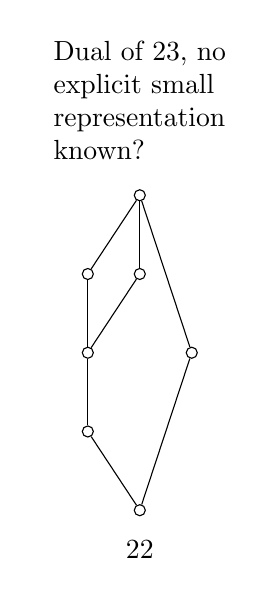
\begin{tikzpicture}
[scale=2, e/.style={circle,draw,inner sep=0pt,minimum size=4pt}]
\node(6) at (0,1)[e]{};
\node(5) at (-0.33,0.5)[e]{};
\node(4) at (0,0.5)[e]{};
\node(3) at (0.33,0)[e]{};
\node(2) at (-0.33,0)[e]{};
\node(1) at (-0.33,-0.5)[e]{};
\node(0) at (0,-1)[e]{};
\node at (0,-1.25){\scs 22};
\node at (0,1.1)[above]{\begin{tabular}{l}
Dual of 23, no\\
explicit small\\
representation\\
known?\end{tabular}};
\node at (0,1.5){};
\draw(5)--(6);
\draw(4)--(6);
\draw(3)--(6);
\draw(2)--(4);
\draw(2)--(5);
\draw(1)--(2);
\draw(0)--(1);
\draw(0)--(3);
\end{tikzpicture}\end{tabular}
\begin{tabular}{l}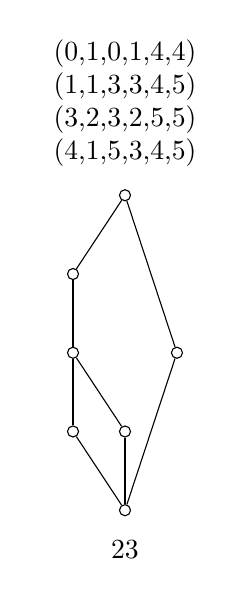
\begin{tikzpicture}
[scale=2, e/.style={circle,draw,inner sep=0pt,minimum size=4pt}]
\node(6) at (0,1)[e]{};
\node(5) at (-0.33,0.5)[e]{};
\node(4) at (-0.33,0)[e]{};
\node(3) at (0.33,0)[e]{};
\node(2) at (-0.33,-0.5)[e]{};
\node(1) at (0,-0.5)[e]{};
\node(0) at (0,-1)[e]{};
\node at (0,-1.25){\scs 23};
\node at (0,1.1)[above]{\begin{tabular}{l}
(0,1,0,1,4,4)\\
(1,1,3,3,4,5)\\
(3,2,3,2,5,5)\\
(4,1,5,3,4,5)
\end{tabular}};
\node at (0,1.5){};
\draw(5)--(6);
\draw(4)--(5);
\draw(3)--(6);
\draw(2)--(4);
\draw(1)--(4);
\draw(0)--(3);
\draw(0)--(2);
\draw(0)--(1);
\end{tikzpicture}\end{tabular}
\begin{tabular}{l}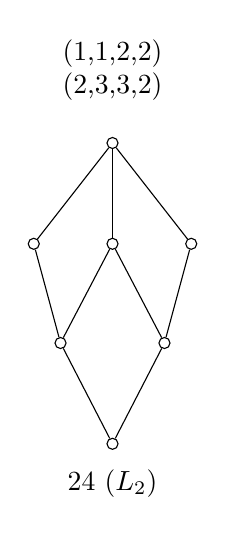
\begin{tikzpicture}
[scale=2, e/.style={circle,draw,inner sep=0pt,minimum size=4pt}]
\node(6) at (-0.0,0.91)[e]{};
\node(5) at (0.0,0.27)[e]{};
\node(4) at (0.5,0.27)[e]{};
\node(3) at (-0.5,0.27)[e]{};
\node(2) at (0.33,-0.36)[e]{};
\node(1) at (-0.33,-0.36)[e]{};
\node(0) at (-0.0,-1.0)[e]{};
\node at (0,-1.25){\scs 24 ($L_2$)};
\node at (0,1.1)[above]{\begin{tabular}{l}
(1,1,2,2)\\
(2,3,3,2)\end{tabular}};
\node at (0,1.5){};
\draw(5)--(6);
\draw(4)--(6);
\draw(3)--(6);
\draw(2)--(4);
\draw(2)--(5);
\draw(1)--(3);
\draw(1)--(5);
\draw(0)--(1);
\draw(0)--(2);
\end{tikzpicture}\end{tabular}
\begin{tabular}{l}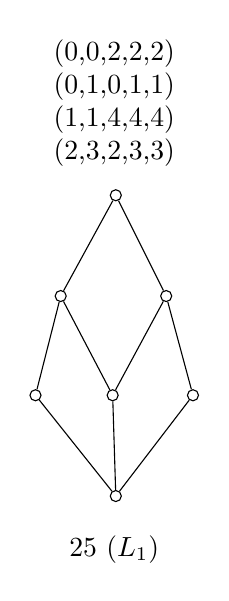
\begin{tikzpicture}
[scale=2, e/.style={circle,draw,inner sep=0pt,minimum size=4pt}]
\node(6) at (0.01,1.0)[e]{};
\node(5) at (-0.34,0.36)[e]{};
\node(4) at (0.33,0.36)[e]{};
\node(3) at (-0.5,-0.27)[e]{};
\node(2) at (0.5,-0.27)[e]{};
\node(1) at (-0.01,-0.27)[e]{};
\node(0) at (0.01,-0.91)[e]{};
\node at (0,-1.25){\scs 25 ($L_1$)};
\node at (0,1.1)[above]{\begin{tabular}{l}
(0,0,2,2,2)\\
(0,1,0,1,1)\\
(1,1,4,4,4)\\
(2,3,2,3,3)\end{tabular}};
\node at (0,1.5){};
\draw(5)--(6);
\draw(4)--(6);
\draw(3)--(5);
\draw(2)--(4);
\draw(1)--(5);
\draw(1)--(4);
\draw(0)--(3);
\draw(0)--(2);
\draw(0)--(1);
\end{tikzpicture}\end{tabular}
\begin{tabular}{l}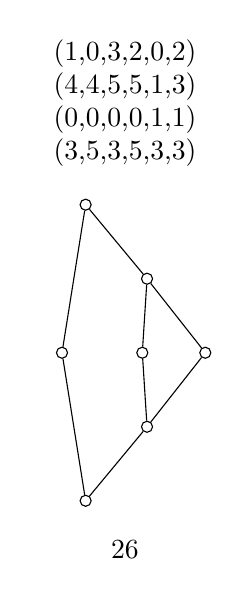
\begin{tikzpicture}
[scale=2, e/.style={circle,draw,inner sep=0pt,minimum size=4pt}]
\node(6) at (-0.25,0.94)[e]{};
\node(5) at (0.14,0.47)[e]{};
\node(4) at (-0.4,0.0)[e]{};
\node(3) at (0.11,0.0)[e]{};
\node(2) at (0.51,0.0)[e]{};
\node(1) at (0.14,-0.47)[e]{};
\node(0) at (-0.25,-0.94)[e]{};
\node at (0,-1.25){\scs 26};
\node at (0,1.1)[above]{\begin{tabular}{l}
(1,0,3,2,0,2)\\
(4,4,5,5,1,3)\\
(0,0,0,0,1,1)\\
(3,5,3,5,3,3)\end{tabular}};
\node at (0,1.5){};
\draw(5)--(6);
\draw(4)--(6);
\draw(3)--(5);
\draw(2)--(5);
\draw(1)--(2);
\draw(1)--(3);
\draw(0)--(1);
\draw(0)--(4);
\end{tikzpicture}\end{tabular}
\begin{tabular}{l}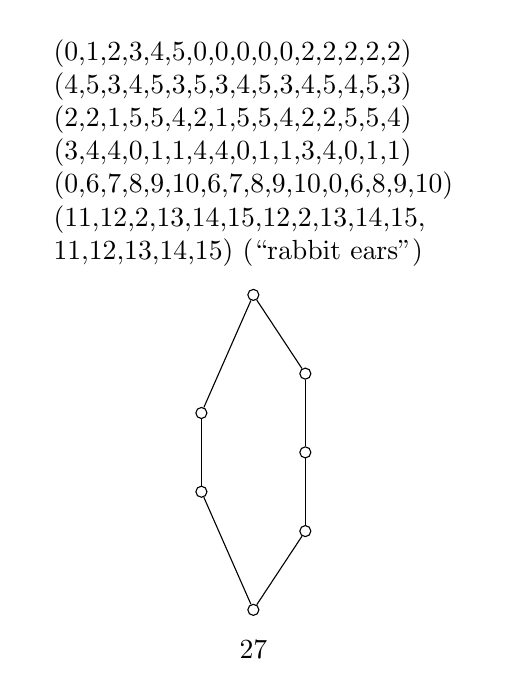
\begin{tikzpicture}
[scale=2, e/.style={circle,draw,inner sep=0pt,minimum size=4pt}]
\node(6) at (0,1)[e]{};
\node(5) at (0.33,0.5)[e]{};
\node(4) at (-0.33,0.25)[e]{};
\node(3) at (0.33,0.0)[e]{};
\node(2) at (-0.33,-0.25)[e]{};
\node(1) at (0.33,-0.5)[e]{};
\node(0) at (0,-1)[e]{};
\node at (0,-1.25){\scs 27};
\node at (0,1.1)[above]{\begin{tabular}{l}
(0,1,2,3,4,5,0,0,0,0,0,2,2,2,2,2)\\
(4,5,3,4,5,3,5,3,4,5,3,4,5,4,5,3)\\
(2,2,1,5,5,4,2,1,5,5,4,2,2,5,5,4)\\
(3,4,4,0,1,1,4,4,0,1,1,3,4,0,1,1)\\
(0,6,7,8,9,10,6,7,8,9,10,0,6,8,9,10)\\
(11,12,2,13,14,15,12,2,13,14,15,\\
11,12,13,14,15) (``rabbit ears'')
\end{tabular}};
\node at (0,1.5){};
\draw(5)--(6);
\draw(4)--(6);
\draw(3)--(5);
\draw(2)--(4);
\draw(1)--(3);
\draw(0)--(1);
\draw(0)--(2);
\end{tikzpicture}\end{tabular}
\begin{tabular}{l}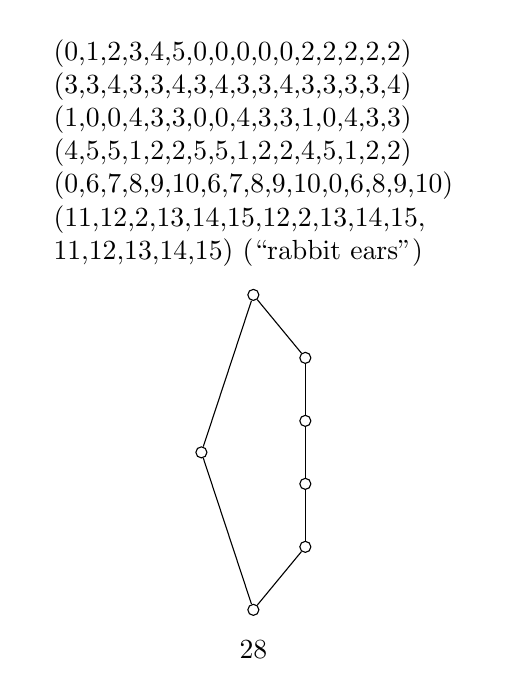
\begin{tikzpicture}
[scale=2, e/.style={circle,draw,inner sep=0pt,minimum size=4pt}]
\node(6) at (0,1)[e]{};
\node(5) at (0.33,0.6)[e]{};
\node(4) at (-0.33,0)[e]{};
\node(3) at (0.33,0.2)[e]{};
\node(2) at (0.33,-0.2)[e]{};
\node(1) at (0.33,-0.6)[e]{};
\node(0) at (0,-1)[e]{};
\node at (0,-1.25){\scs 28};
\node at (0,1.1)[above]{\begin{tabular}{l}
(0,1,2,3,4,5,0,0,0,0,0,2,2,2,2,2)\\
(3,3,4,3,3,4,3,4,3,3,4,3,3,3,3,4)\\
(1,0,0,4,3,3,0,0,4,3,3,1,0,4,3,3)\\
(4,5,5,1,2,2,5,5,1,2,2,4,5,1,2,2)\\
(0,6,7,8,9,10,6,7,8,9,10,0,6,8,9,10)\\
(11,12,2,13,14,15,12,2,13,14,15,\\
11,12,13,14,15) (``rabbit ears'')
\end{tabular}};
\node at (0,1.5){};
\draw(5)--(6);
\draw(4)--(6);
\draw(3)--(5);
\draw(2)--(3);
\draw(1)--(2);
\draw(0)--(1);
\draw(0)--(4);
\end{tikzpicture}\end{tabular}
\begin{tabular}{l}\begin{tikzpicture}
[scale=2, e/.style={circle,draw,inner sep=0pt,minimum size=4pt}]
\node(6) at (-0.19,0.98)[e]{};
\node(5) at (0.38,0.49)[e]{};
\node(4) at (-0.25,0.25)[e]{};
\node(3) at (0.63,0.0)[e]{};
\node(2) at (-0.52,-0.25)[e]{};
\node(1) at (0.15,-0.49)[e]{};
\node(0) at (-0.19,-0.98)[e]{};
\node at (0,-1.25){\scs 29};
\node at (0,1.1)[above]{\begin{tabular}{l}
(1,0,3,2,2)\\
(2,4,2,4,3)\end{tabular}};
\node at (0,1.5){};
\draw(5)--(6);
\draw(4)--(6);
\draw(3)--(5);
\draw(2)--(4);
\draw(1)--(3);
\draw(1)--(4);
\draw(0)--(1);
\draw(0)--(2);
\end{tikzpicture}\end{tabular}
\begin{tabular}{l}\begin{tikzpicture}
[scale=2, e/.style={circle,draw,inner sep=0pt,minimum size=4pt}]
\node(6) at (-0.19,0.98)[e]{};
\node(5) at (0.15,0.49)[e]{};
\node(4) at (-0.52,0.25)[e]{};
\node(3) at (0.63,0.0)[e]{};
\node(2) at (-0.25,-0.25)[e]{};
\node(1) at (0.38,-0.49)[e]{};
\node(0) at (-0.19,-0.98)[e]{};
\node at (0,-1.25){\scs 30};
\node at (0,1.1)[above]{\begin{tabular}{l}
(0,3,4,3,4)\\
(2,2,1,4,3)\end{tabular}};
\node at (0,1.5){};
\draw(5)--(6);
\draw(4)--(6);
\draw(3)--(5);
\draw(2)--(5);
\draw(2)--(4);
\draw(1)--(3);
\draw(0)--(2);
\draw(0)--(1);
\end{tikzpicture}\end{tabular}
\begin{tabular}{l}\begin{tikzpicture}
[scale=2, e/.style={circle,draw,inner sep=0pt,minimum size=4pt}]
\node(6) at (0.09,0.99)[e]{};
\node(5) at (-0.3,0.51)[e]{};
\node(4) at (0.43,0.27)[e]{};
\node(3) at (-0.21,0.03)[e]{};
\node(2) at (-0.37,-0.45)[e]{};
\node(1) at (0.27,-0.45)[e]{};
\node(0) at (0.09,-0.93)[e]{};
\node at (0,-1.25){\scs 31};
\node at (0,1.1)[above]{\begin{tabular}{l}
(0,1,1,0,0)\\
(1,1,2,2,2)\\
(3,2,2,4,4)\end{tabular}};
\node at (0,1.5){};
\draw(5)--(6);
\draw(4)--(6);
\draw(3)--(5);
\draw(2)--(3);
\draw(1)--(3);
\draw(1)--(4);
\draw(0)--(1);
\draw(0)--(2);
\end{tikzpicture}\end{tabular}
\begin{tabular}{l}\begin{tikzpicture}
[scale=2, e/.style={circle,draw,inner sep=0pt,minimum size=4pt}]
\node(6) at (0.09,0.93)[e]{};
\node(5) at (0.28,0.45)[e]{};
\node(4) at (-0.37,0.45)[e]{};
\node(3) at (-0.2,-0.03)[e]{};
\node(2) at (0.44,-0.27)[e]{};
\node(1) at (-0.32,-0.52)[e]{};
\node(0) at (0.09,-1.0)[e]{};
\node at (0,-1.25){\scs 32};
\node at (0,1.1)[above]{\begin{tabular}{l}
(0,1,1,3,3)\\
(1,2,2,4,4)\\
(3,3,4,3,4)
\end{tabular}};
\node at (0,1.5){};
\draw(5)--(6);
\draw(4)--(6);
\draw(3)--(5);
\draw(3)--(4);
\draw(2)--(5);
\draw(1)--(3);
\draw(0)--(2);
\draw(0)--(1);
\end{tikzpicture}\end{tabular}
\begin{tabular}{l}\begin{tikzpicture}
[scale=2, e/.style={circle,draw,inner sep=0pt,minimum size=4pt}]
\node(6) at (0.0,1.0)[e]{};
\node(5) at (-0.41,0.0)[e]{};
\node(4) at (0.25,0.0)[e]{};
\node(3) at (0.0,0.0)[e]{};
\node(2) at (-0.25,0.0)[e]{};
\node(1) at (0.41,0.0)[e]{};
\node(0) at (0.0,-1.0)[e]{};
\node at (0,-1.25){\scs 33 $(M_5)$};
\node at (0,1.1)[above]{\begin{tabular}{l}
(1,3,2,0,9,11,10,8,13,15,14,12,5,7,6,4)\\
(11,8,10,9,7,4,6,5,15,12,14,13,3,0,2,1)\\
(14,15,12,13,10,11,8,9,6,7,4,5,2,3,0,1)\end{tabular}};
\node at (0,1.5){};
\draw(5)--(6);
\draw(4)--(6);
\draw(3)--(6);
\draw(2)--(6);
\draw(1)--(6);
\draw(0)--(1);
\draw(0)--(2);
\draw(0)--(3);
\draw(0)--(4);
\draw(0)--(5);
\end{tikzpicture}\end{tabular}
\begin{tabular}{l}\begin{tikzpicture}
[scale=2, e/.style={circle,draw,inner sep=0pt,minimum size=4pt}]
\node(6) at (0.0,0.91)[e]{};
\node(5) at (0.24,0.27)[e]{};
\node(4) at (-0.42,0.27)[e]{};
\node(3) at (-0.08,0.27)[e]{};
\node(2) at (0.39,-0.36)[e]{};
\node(1) at (-0.13,-0.36)[e]{};
\node(0) at (0.0,-1.0)[e]{};
\node at (0,-1.25){\scs 34};
\node at (0,1.1)[above]{\begin{tabular}{l}
(0,1,3,2)\end{tabular}};
\node at (0,1.5){};
\draw(5)--(6);
\draw(4)--(6);
\draw(3)--(6);
\draw(2)--(5);
\draw(1)--(3);
\draw(1)--(4);
\draw(1)--(5);
\draw(0)--(1);
\draw(0)--(2);
\end{tikzpicture}\end{tabular}
\begin{tabular}{l}\begin{tikzpicture}
[scale=2, e/.style={circle,draw,inner sep=0pt,minimum size=4pt}]
\node(6) at (0.01,1.0)[e]{};
\node(5) at (-0.14,0.36)[e]{};
\node(4) at (0.4,0.36)[e]{};
\node(3) at (-0.41,-0.27)[e]{};
\node(2) at (-0.1,-0.27)[e]{};
\node(1) at (0.24,-0.27)[e]{};
\node(0) at (0.01,-0.91)[e]{};
\node at (0,-1.25){\scs 35};
\node at (0,1.1)[above]{\begin{tabular}{l}
(1,1,2,3)\\
(2,3,3,3)\end{tabular}};
\node at (0,1.5){};
\draw(5)--(6);
\draw(4)--(6);
\draw(3)--(5);
\draw(2)--(5);
\draw(1)--(5);
\draw(1)--(4);
\draw(0)--(3);
\draw(0)--(2);
\draw(0)--(1);
\end{tikzpicture}\end{tabular}
%\end{document}

